I present some stylized facts that motivate the puzzle and the hypothesized link between FDI and corruption:

\begin{itemize}
	\item The spillover effect of FDI on growth is highly variable. For example, FDI is found to be growth-enhancing in East Asia, but not in Latin America \citep{Zhang2001}. Similarly, the effect of FDI on domestic investment also varies across countries and regions. FDI is found to crowd in investment in some countries (e.g. Ghana, Senegal, South Korea, Pakistan, Thailand, etc.) but crowd out in others \citep{Agosin2005}.
	
	\item Despite the prevalent concern with discrimination against foreign firms in the international business literature, the World Bank Enterprise Survey finds that foreign firms actually face fewer obstacles than domestic firms while doing business, suggesting a collusive relationship between host governments and foreign firms \citep{Batra2003}.
	
	\item The correlation between corruption and FDI is negative. However, there is a lot of unexplained variance at the high end of FDI. Countries with high level of FDI run the gamut of corruption (\Cref{fig:fdi_corruption}).
	
	\begin{figure}[!ht]
	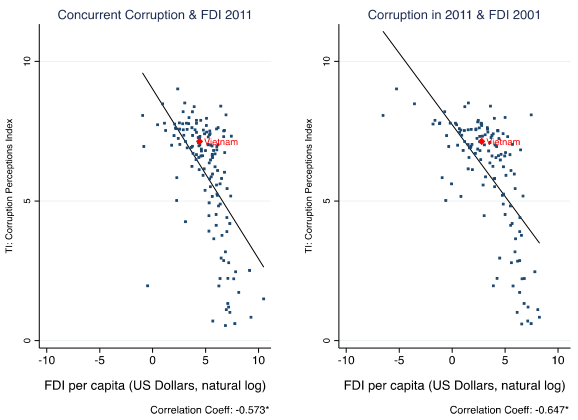
\includegraphics[width=\textwidth, height=\textheight,keepaspectratio]{../figure/fdi_corruption}
	\caption{Source: \citep{Malesky2015}}
	\label{fig:fdi_corruption}
	\end{figure}
\end{itemize}
